\documentclass[1p]{elsarticle_modified}
%\bibliographystyle{elsarticle-num}

%\usepackage[colorlinks]{hyperref}
%\usepackage{abbrmath_seonhwa} %\Abb, \Ascr, \Acal ,\Abf, \Afrak
\usepackage{amsfonts}
\usepackage{amssymb}
\usepackage{amsmath}
\usepackage{amsthm}
\usepackage{scalefnt}
\usepackage{amsbsy}
\usepackage{kotex}
\usepackage{caption}
\usepackage{subfig}
\usepackage{color}
\usepackage{graphicx}
\usepackage{xcolor} %% white, black, red, green, blue, cyan, magenta, yellow
\usepackage{float}
\usepackage{setspace}
\usepackage{hyperref}

\usepackage{tikz}
\usetikzlibrary{arrows}

\usepackage{multirow}
\usepackage{array} % fixed length table
\usepackage{hhline}

%%%%%%%%%%%%%%%%%%%%%
\makeatletter
\renewcommand*\env@matrix[1][\arraystretch]{%
	\edef\arraystretch{#1}%
	\hskip -\arraycolsep
	\let\@ifnextchar\new@ifnextchar
	\array{*\c@MaxMatrixCols c}}
\makeatother %https://tex.stackexchange.com/questions/14071/how-can-i-increase-the-line-spacing-in-a-matrix
%%%%%%%%%%%%%%%

\usepackage[normalem]{ulem}

\newcommand{\msout}[1]{\ifmmode\text{\sout{\ensuremath{#1}}}\else\sout{#1}\fi}
%SOURCE: \msout is \stkout macro in https://tex.stackexchange.com/questions/20609/strikeout-in-math-mode

\newcommand{\cancel}[1]{
	\ifmmode
	{\color{red}\msout{#1}}
	\else
	{\color{red}\sout{#1}}
	\fi
}

\newcommand{\add}[1]{
	{\color{blue}\uwave{#1}}
}

\newcommand{\replace}[2]{
	\ifmmode
	{\color{red}\msout{#1}}{\color{blue}\uwave{#2}}
	\else
	{\color{red}\sout{#1}}{\color{blue}\uwave{#2}}
	\fi
}

\newcommand{\Sol}{\mathcal{S}} %segment
\newcommand{\D}{D} %diagram
\newcommand{\A}{\mathcal{A}} %arc


%%%%%%%%%%%%%%%%%%%%%%%%%%%%%5 test

\def\sl{\operatorname{\textup{SL}}(2,\Cbb)}
\def\psl{\operatorname{\textup{PSL}}(2,\Cbb)}
\def\quan{\mkern 1mu \triangleright \mkern 1mu}

\theoremstyle{definition}
\newtheorem{thm}{Theorem}[section]
\newtheorem{prop}[thm]{Proposition}
\newtheorem{lem}[thm]{Lemma}
\newtheorem{ques}[thm]{Question}
\newtheorem{cor}[thm]{Corollary}
\newtheorem{defn}[thm]{Definition}
\newtheorem{exam}[thm]{Example}
\newtheorem{rmk}[thm]{Remark}
\newtheorem{alg}[thm]{Algorithm}

\newcommand{\I}{\sqrt{-1}}
\begin{document}

%\begin{frontmatter}
%
%\title{Boundary parabolic representations of knots up to 8 crossings}
%
%%% Group authors per affiliation:
%\author{Yunhi Cho} 
%\address{Department of Mathematics, University of Seoul, Seoul, Korea}
%\ead{yhcho@uos.ac.kr}
%
%
%\author{Seonhwa Kim} %\fnref{s_kim}}
%\address{Center for Geometry and Physics, Institute for Basic Science, Pohang, 37673, Korea}
%\ead{ryeona17@ibs.re.kr}
%
%\author{Hyuk Kim}
%\address{Department of Mathematical Sciences, Seoul National University, Seoul 08826, Korea}
%\ead{hyukkim@snu.ac.kr}
%
%\author{Seokbeom Yoon}
%\address{Department of Mathematical Sciences, Seoul National University, Seoul, 08826,  Korea}
%\ead{sbyoon15@snu.ac.kr}
%
%\begin{abstract}
%We find all boundary parabolic representation of knots up to 8 crossings.
%
%\end{abstract}
%\begin{keyword}
%    \MSC[2010] 57M25 
%\end{keyword}
%
%\end{frontmatter}

%\linenumbers
%\tableofcontents
%
\newcommand\colored[1]{\textcolor{white}{\rule[-0.35ex]{0.8em}{1.4ex}}\kern-0.8em\color{red} #1}%
%\newcommand\colored[1]{\textcolor{white}{ #1}\kern-2.17ex	\textcolor{white}{ #1}\kern-1.81ex	\textcolor{white}{ #1}\kern-2.15ex\color{red}#1	}

{\Large $\underline{10_{53}~(K10a_{14})}$}

\setlength{\tabcolsep}{10pt}
\renewcommand{\arraystretch}{1.6}
\vspace{1cm}\begin{tabular}{m{100pt}>{\centering\arraybackslash}m{274pt}}
\multirow{5}{120pt}{
	\centering
	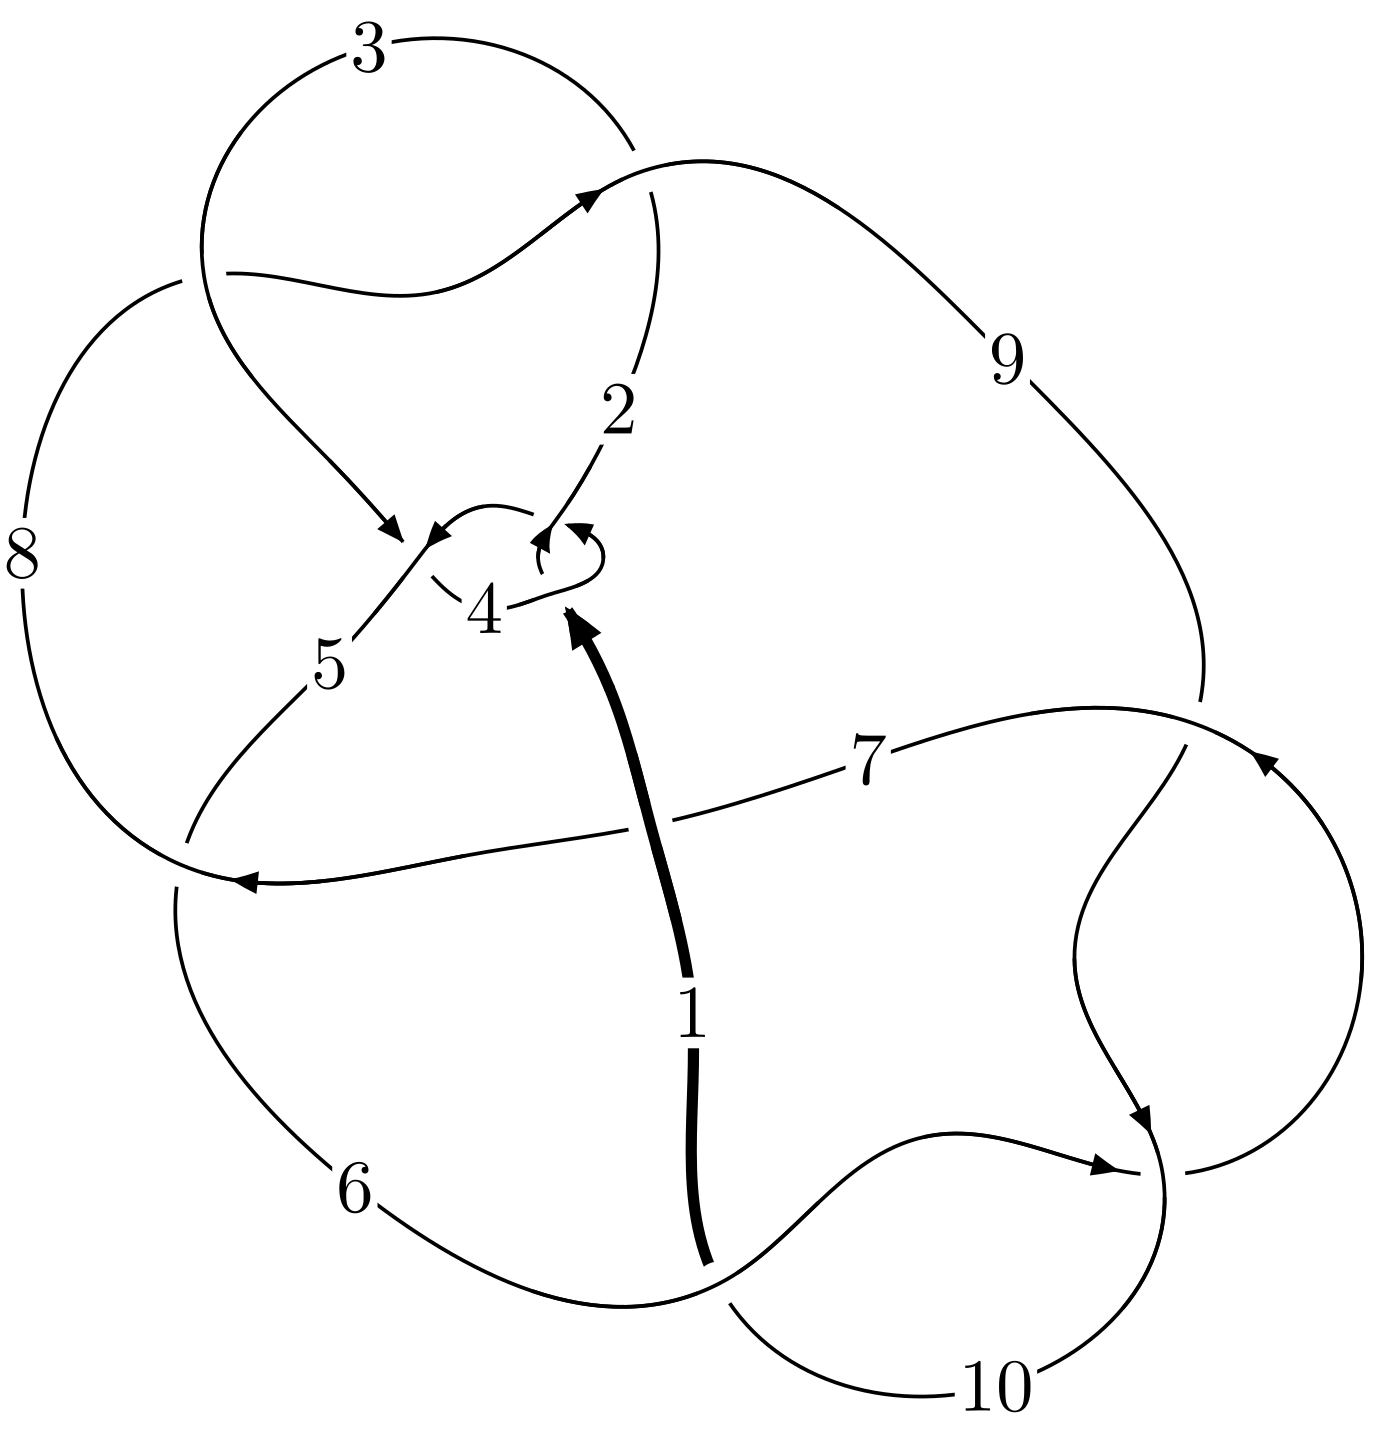
\includegraphics[width=112pt]{../../../GIT/diagram.site/Diagrams/png/137_10_53.png}\\
\ \ \ A knot diagram\footnotemark}&
\allowdisplaybreaks
\textbf{Linearized knot diagam} \\
\cline{2-2}
 &
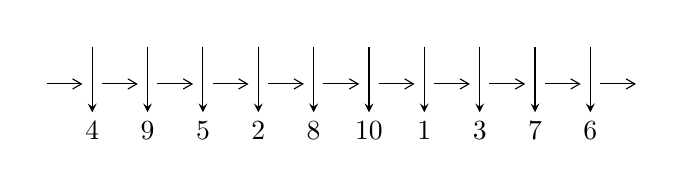
\begin{tikzpicture}[x=20pt, y=17pt]
	% nodes
	\node (C0) at (0, 0) {};
	\node (C1) at (1, 0) {};
	\node (C1U) at (1, +1) {};
	\node (C1D) at (1, -1) {4};

	\node (C2) at (2, 0) {};
	\node (C2U) at (2, +1) {};
	\node (C2D) at (2, -1) {9};

	\node (C3) at (3, 0) {};
	\node (C3U) at (3, +1) {};
	\node (C3D) at (3, -1) {5};

	\node (C4) at (4, 0) {};
	\node (C4U) at (4, +1) {};
	\node (C4D) at (4, -1) {2};

	\node (C5) at (5, 0) {};
	\node (C5U) at (5, +1) {};
	\node (C5D) at (5, -1) {8};

	\node (C6) at (6, 0) {};
	\node (C6U) at (6, +1) {};
	\node (C6D) at (6, -1) {10};

	\node (C7) at (7, 0) {};
	\node (C7U) at (7, +1) {};
	\node (C7D) at (7, -1) {1};

	\node (C8) at (8, 0) {};
	\node (C8U) at (8, +1) {};
	\node (C8D) at (8, -1) {3};

	\node (C9) at (9, 0) {};
	\node (C9U) at (9, +1) {};
	\node (C9D) at (9, -1) {7};

	\node (C10) at (10, 0) {};
	\node (C10U) at (10, +1) {};
	\node (C10D) at (10, -1) {6};
	\node (C11) at (11, 0) {};

	% arrows
	\draw[->,>={angle 60}]
	(C0) edge (C1) (C1) edge (C2) (C2) edge (C3) (C3) edge (C4) (C4) edge (C5) (C5) edge (C6) (C6) edge (C7) (C7) edge (C8) (C8) edge (C9) (C9) edge (C10) (C10) edge (C11) ;	\draw[->,>=stealth]
	(C1U) edge (C1D) (C2U) edge (C2D) (C3U) edge (C3D) (C4U) edge (C4D) (C5U) edge (C5D) (C6U) edge (C6D) (C7U) edge (C7D) (C8U) edge (C8D) (C9U) edge (C9D) (C10U) edge (C10D) ;
	\end{tikzpicture} \\
\hhline{~~} \\& 
\textbf{Solving Sequence} \\ \cline{2-2} 
 &
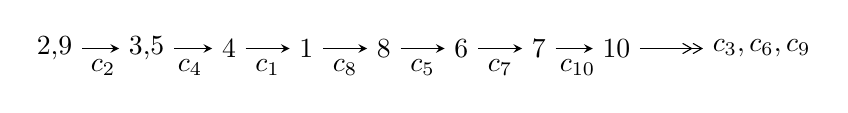
\begin{tikzpicture}[x=28pt, y=7pt]
	% node
	\node (A0) at (-1/8, 0) {2,9};
	\node (A1) at (17/16, 0) {3,5};
	\node (A2) at (17/8, 0) {4};
	\node (A3) at (25/8, 0) {1};
	\node (A4) at (33/8, 0) {8};
	\node (A5) at (41/8, 0) {6};
	\node (A6) at (49/8, 0) {7};
	\node (A7) at (57/8, 0) {10};
	\node (C1) at (1/2, -1) {$c_{2}$};
	\node (C2) at (13/8, -1) {$c_{4}$};
	\node (C3) at (21/8, -1) {$c_{1}$};
	\node (C4) at (29/8, -1) {$c_{8}$};
	\node (C5) at (37/8, -1) {$c_{5}$};
	\node (C6) at (45/8, -1) {$c_{7}$};
	\node (C7) at (53/8, -1) {$c_{10}$};
	\node (A8) at (9, 0) {$c_{3},c_{6},c_{9}$};

	% edge
	\draw[->,>=stealth]	
	(A0) edge (A1) (A1) edge (A2) (A2) edge (A3) (A3) edge (A4) (A4) edge (A5) (A5) edge (A6) (A6) edge (A7) ;
	\draw[->>,>={angle 60}]	
	(A7) edge (A8);
\end{tikzpicture} \\ 

\end{tabular} \\

\footnotetext{
The image of knot diagram is generated by the software ``\textbf{Draw programme}" developed by Andrew Bartholomew(\url{http://www.layer8.co.uk/maths/draw/index.htm\#Running-draw}), where we modified some parts for our purpose(\url{https://github.com/CATsTAILs/LinksPainter}).
}\phantom \\ \newline 
\centering \textbf{Ideals for irreducible components\footnotemark of $X_{\text{par}}$} 
 
\begin{align*}
I^u_{1}&=\langle 
-1.00600\times10^{29} u^{38}+2.48316\times10^{29} u^{37}+\cdots+8.64881\times10^{29} b+3.57482\times10^{30},\\
\phantom{I^u_{1}}&\phantom{= \langle  }1.23985\times10^{30} u^{38}+2.03123\times10^{29} u^{37}+\cdots+3.45952\times10^{30} a-6.27933\times10^{30},\;u^{39}+u^{38}+\cdots+20 u+8\rangle \\
\\
I^v_{1}&=\langle 
a,\;b-1,\;v^3- v^2+1\rangle \\
\end{align*}
\raggedright * 2 irreducible components of $\dim_{\mathbb{C}}=0$, with total 42 representations.\\
\footnotetext{All coefficients of polynomials are rational numbers. But the coefficients are sometimes approximated in decimal forms when there is not enough margin.}
\newpage
\renewcommand{\arraystretch}{1}
\centering \section*{I. $I^u_{1}= \langle -1.01\times10^{29} u^{38}+2.48\times10^{29} u^{37}+\cdots+8.65\times10^{29} b+3.57\times10^{30},\;1.24\times10^{30} u^{38}+2.03\times10^{29} u^{37}+\cdots+3.46\times10^{30} a-6.28\times10^{30},\;u^{39}+u^{38}+\cdots+20 u+8 \rangle$}
\flushleft \textbf{(i) Arc colorings}\\
\begin{tabular}{m{7pt} m{180pt} m{7pt} m{180pt} }
\flushright $a_{2}=$&$\begin{pmatrix}1\\0\end{pmatrix}$ \\
\flushright $a_{9}=$&$\begin{pmatrix}0\\u\end{pmatrix}$ \\
\flushright $a_{3}=$&$\begin{pmatrix}1\\u^2\end{pmatrix}$ \\
\flushright $a_{5}=$&$\begin{pmatrix}-0.358388 u^{38}-0.0587140 u^{37}+\cdots-1.78450 u+1.81508\\0.116317 u^{38}-0.287110 u^{37}+\cdots-9.31854 u-4.13331\end{pmatrix}$ \\
\flushright $a_{4}=$&$\begin{pmatrix}-0.242071 u^{38}-0.345824 u^{37}+\cdots-11.1030 u-2.31823\\0.116317 u^{38}-0.287110 u^{37}+\cdots-9.31854 u-4.13331\end{pmatrix}$ \\
\flushright $a_{1}=$&$\begin{pmatrix}-0.241767 u^{38}+0.162227 u^{37}+\cdots+4.40767 u+3.55101\\0.116621 u^{38}+0.220941 u^{37}+\cdots+6.19217 u+1.73592\end{pmatrix}$ \\
\flushright $a_{8}=$&$\begin{pmatrix}u\\u^3+u\end{pmatrix}$ \\
\flushright $a_{6}=$&$\begin{pmatrix}-0.242918 u^{38}-0.232042 u^{37}+\cdots-7.93025 u-1.41687\\0.221145 u^{38}-0.326120 u^{37}+\cdots-10.6121 u-5.05488\end{pmatrix}$ \\
\flushright $a_{7}=$&$\begin{pmatrix}-0.198873 u^{38}-0.0970595 u^{37}+\cdots+1.83795 u+1.62354\\0.233523 u^{38}-0.0483612 u^{37}+\cdots+1.48213 u-1.84886\end{pmatrix}$ \\
\flushright $a_{10}=$&$\begin{pmatrix}-0.153182 u^{38}-0.312103 u^{37}+\cdots-7.28402 u-2.56081\\0.660384 u^{38}+0.789150 u^{37}+\cdots+16.3791 u+4.59908\end{pmatrix}$\\&\end{tabular}
\flushleft \textbf{(ii) Obstruction class $= -1$}\\~\\
\flushleft \textbf{(iii) Cusp Shapes $= -0.333316 u^{38}-0.171100 u^{37}+\cdots+10.6866 u-4.74934$}\\~\\
\newpage\renewcommand{\arraystretch}{1}
\flushleft \textbf{(iv) u-Polynomials at the component}\newline \\
\begin{tabular}{m{50pt}|m{274pt}}
Crossings & \hspace{64pt}u-Polynomials at each crossing \\
\hline $$\begin{aligned}c_{1},c_{4}\end{aligned}$$&$\begin{aligned}
&u^{39}-4 u^{38}+\cdots+u+1
\end{aligned}$\\
\hline $$\begin{aligned}c_{2},c_{8}\end{aligned}$$&$\begin{aligned}
&u^{39}+u^{38}+\cdots+20 u+8
\end{aligned}$\\
\hline $$\begin{aligned}c_{3}\end{aligned}$$&$\begin{aligned}
&u^{39}+18 u^{38}+\cdots+17 u+1
\end{aligned}$\\
\hline $$\begin{aligned}c_{5}\end{aligned}$$&$\begin{aligned}
&u^{39}-8 u^{38}+\cdots-168 u+49
\end{aligned}$\\
\hline $$\begin{aligned}c_{6},c_{9},c_{10}\end{aligned}$$&$\begin{aligned}
&u^{39}-2 u^{38}+\cdots-4 u^2+1
\end{aligned}$\\
\hline $$\begin{aligned}c_{7}\end{aligned}$$&$\begin{aligned}
&u^{39}+2 u^{38}+\cdots+6 u+9
\end{aligned}$\\
\hline
\end{tabular}\\~\\
\newpage\renewcommand{\arraystretch}{1}
\flushleft \textbf{(v) Riley Polynomials at the component}\newline \\
\begin{tabular}{m{50pt}|m{274pt}}
Crossings & \hspace{64pt}Riley Polynomials at each crossing \\
\hline $$\begin{aligned}c_{1},c_{4}\end{aligned}$$&$\begin{aligned}
&y^{39}-18 y^{38}+\cdots+17 y-1
\end{aligned}$\\
\hline $$\begin{aligned}c_{2},c_{8}\end{aligned}$$&$\begin{aligned}
&y^{39}+21 y^{38}+\cdots-304 y-64
\end{aligned}$\\
\hline $$\begin{aligned}c_{3}\end{aligned}$$&$\begin{aligned}
&y^{39}+10 y^{38}+\cdots+273 y-1
\end{aligned}$\\
\hline $$\begin{aligned}c_{5}\end{aligned}$$&$\begin{aligned}
&y^{39}+16 y^{38}+\cdots-14896 y-2401
\end{aligned}$\\
\hline $$\begin{aligned}c_{6},c_{9},c_{10}\end{aligned}$$&$\begin{aligned}
&y^{39}+36 y^{38}+\cdots+8 y-1
\end{aligned}$\\
\hline $$\begin{aligned}c_{7}\end{aligned}$$&$\begin{aligned}
&y^{39}+4 y^{38}+\cdots-648 y-81
\end{aligned}$\\
\hline
\end{tabular}\\~\\
\newpage\flushleft \textbf{(vi) Complex Volumes and Cusp Shapes}
$$\begin{array}{c|c|c}  
\text{Solutions to }I^u_{1}& \I (\text{vol} + \sqrt{-1}CS) & \text{Cusp shape}\\
 \hline 
\begin{aligned}
u &= \phantom{-}1.017070 + 0.016485 I \\
a &= \phantom{-}0.533352 + 0.181785 I \\
b &= \phantom{-}0.679795 - 0.572535 I\end{aligned}
 & \phantom{-}4.66283 - 1.97475 I & -5.44784 + 0.24565 I \\ \hline\begin{aligned}
u &= \phantom{-}1.017070 - 0.016485 I \\
a &= \phantom{-}0.533352 - 0.181785 I \\
b &= \phantom{-}0.679795 + 0.572535 I\end{aligned}
 & \phantom{-}4.66283 + 1.97475 I & -5.44784 - 0.24565 I \\ \hline\begin{aligned}
u &= -0.231699 + 0.952667 I \\
a &= \phantom{-}0.433679 - 0.020477 I \\
b &= \phantom{-}1.300720 + 0.108633 I\end{aligned}
 & \phantom{-}2.67862 + 4.04441 I & -5.85906 - 4.24790 I \\ \hline\begin{aligned}
u &= -0.231699 - 0.952667 I \\
a &= \phantom{-}0.433679 + 0.020477 I \\
b &= \phantom{-}1.300720 - 0.108633 I\end{aligned}
 & \phantom{-}2.67862 - 4.04441 I & -5.85906 + 4.24790 I \\ \hline\begin{aligned}
u &= \phantom{-}0.956761 + 0.380033 I \\
a &= \phantom{-}0.481763 + 0.120619 I \\
b &= \phantom{-}0.953268 - 0.489041 I\end{aligned}
 & -1.62662 + 3.39278 I & -12.11270 - 5.92716 I \\ \hline\begin{aligned}
u &= \phantom{-}0.956761 - 0.380033 I \\
a &= \phantom{-}0.481763 - 0.120619 I \\
b &= \phantom{-}0.953268 + 0.489041 I\end{aligned}
 & -1.62662 - 3.39278 I & -12.11270 + 5.92716 I \\ \hline\begin{aligned}
u &= -0.446453 + 0.963476 I \\
a &= \phantom{-}0.00685 - 2.03156 I \\
b &= -0.998340 + 0.492226 I\end{aligned}
 & \phantom{-}1.05258 + 5.41055 I & -8.42668 - 7.07273 I \\ \hline\begin{aligned}
u &= -0.446453 - 0.963476 I \\
a &= \phantom{-}0.00685 + 2.03156 I \\
b &= -0.998340 - 0.492226 I\end{aligned}
 & \phantom{-}1.05258 - 5.41055 I & -8.42668 + 7.07273 I \\ \hline\begin{aligned}
u &= \phantom{-}0.313799 + 0.869843 I \\
a &= \phantom{-}0.49321 + 2.23303 I \\
b &= -0.905691 - 0.426992 I\end{aligned}
 & -2.15141 - 1.70381 I & -11.63741 + 3.75866 I \\ \hline\begin{aligned}
u &= \phantom{-}0.313799 - 0.869843 I \\
a &= \phantom{-}0.49321 - 2.23303 I \\
b &= -0.905691 + 0.426992 I\end{aligned}
 & -2.15141 + 1.70381 I & -11.63741 - 3.75866 I\\
 \hline 
 \end{array}$$\newpage$$\begin{array}{c|c|c}  
\text{Solutions to }I^u_{1}& \I (\text{vol} + \sqrt{-1}CS) & \text{Cusp shape}\\
 \hline 
\begin{aligned}
u &= -0.654305 + 0.610659 I \\
a &= \phantom{-}0.464054 - 0.067479 I \\
b &= \phantom{-}1.110300 + 0.306863 I\end{aligned}
 & -0.106397 - 1.133730 I & -10.95849 + 0.14045 I \\ \hline\begin{aligned}
u &= -0.654305 - 0.610659 I \\
a &= \phantom{-}0.464054 + 0.067479 I \\
b &= \phantom{-}1.110300 - 0.306863 I\end{aligned}
 & -0.106397 + 1.133730 I & -10.95849 - 0.14045 I \\ \hline\begin{aligned}
u &= -1.078760 + 0.377362 I \\
a &= \phantom{-}0.470618 - 0.137655 I \\
b &= \phantom{-}0.957399 + 0.572535 I\end{aligned}
 & \phantom{-}3.81328 - 6.57302 I & -7.10620 + 5.57627 I \\ \hline\begin{aligned}
u &= -1.078760 - 0.377362 I \\
a &= \phantom{-}0.470618 + 0.137655 I \\
b &= \phantom{-}0.957399 - 0.572535 I\end{aligned}
 & \phantom{-}3.81328 + 6.57302 I & -7.10620 - 5.57627 I \\ \hline\begin{aligned}
u &= \phantom{-}0.287457 + 0.756867 I \\
a &= \phantom{-}0.451557 + 0.026551 I \\
b &= \phantom{-}1.206930 - 0.129766 I\end{aligned}
 & -2.53592 - 1.13990 I & -11.07531 + 5.95720 I \\ \hline\begin{aligned}
u &= \phantom{-}0.287457 - 0.756867 I \\
a &= \phantom{-}0.451557 - 0.026551 I \\
b &= \phantom{-}1.206930 + 0.129766 I\end{aligned}
 & -2.53592 + 1.13990 I & -11.07531 - 5.95720 I \\ \hline\begin{aligned}
u &= -0.194269 + 0.773271 I \\
a &= \phantom{-}1.21955 - 2.26240 I \\
b &= -0.815381 + 0.342489 I\end{aligned}
 & \phantom{-}2.08468 - 1.94841 I & -5.31413 - 1.52369 I \\ \hline\begin{aligned}
u &= -0.194269 - 0.773271 I \\
a &= \phantom{-}1.21955 + 2.26240 I \\
b &= -0.815381 - 0.342489 I\end{aligned}
 & \phantom{-}2.08468 + 1.94841 I & -5.31413 + 1.52369 I \\ \hline\begin{aligned}
u &= -0.770646 + 0.144014 I \\
a &= \phantom{-}0.545673 - 0.103341 I \\
b &= \phantom{-}0.769146 + 0.335047 I\end{aligned}
 & -0.798777 - 0.294565 I & -9.95022 - 1.12683 I \\ \hline\begin{aligned}
u &= -0.770646 - 0.144014 I \\
a &= \phantom{-}0.545673 + 0.103341 I \\
b &= \phantom{-}0.769146 - 0.335047 I\end{aligned}
 & -0.798777 + 0.294565 I & -9.95022 + 1.12683 I\\
 \hline 
 \end{array}$$\newpage$$\begin{array}{c|c|c}  
\text{Solutions to }I^u_{1}& \I (\text{vol} + \sqrt{-1}CS) & \text{Cusp shape}\\
 \hline 
\begin{aligned}
u &= \phantom{-}0.243035 + 1.196980 I \\
a &= \phantom{-}0.558338 - 0.947938 I \\
b &= -0.538688 + 0.783208 I\end{aligned}
 & \phantom{-}3.77660 + 0.24936 I & -5.00470 - 2.68648 I \\ \hline\begin{aligned}
u &= \phantom{-}0.243035 - 1.196980 I \\
a &= \phantom{-}0.558338 + 0.947938 I \\
b &= -0.538688 - 0.783208 I\end{aligned}
 & \phantom{-}3.77660 - 0.24936 I & -5.00470 + 2.68648 I \\ \hline\begin{aligned}
u &= \phantom{-}0.541726 + 0.535219 I \\
a &= \phantom{-}0.814600 - 0.384225 I \\
b &= \phantom{-}0.004189 + 0.473649 I\end{aligned}
 & \phantom{-}3.03156 - 1.95518 I & -5.07609 + 3.73688 I \\ \hline\begin{aligned}
u &= \phantom{-}0.541726 - 0.535219 I \\
a &= \phantom{-}0.814600 + 0.384225 I \\
b &= \phantom{-}0.004189 - 0.473649 I\end{aligned}
 & \phantom{-}3.03156 + 1.95518 I & -5.07609 - 3.73688 I \\ \hline\begin{aligned}
u &= -0.406069 + 1.207170 I \\
a &= \phantom{-}0.543323 + 0.815855 I \\
b &= -0.434521 - 0.849125 I\end{aligned}
 & \phantom{-}3.06039 + 3.68428 I & -6.85695 - 4.07509 I \\ \hline\begin{aligned}
u &= -0.406069 - 1.207170 I \\
a &= \phantom{-}0.543323 - 0.815855 I \\
b &= -0.434521 + 0.849125 I\end{aligned}
 & \phantom{-}3.06039 - 3.68428 I & -6.85695 + 4.07509 I \\ \hline\begin{aligned}
u &= -0.523733 + 1.187360 I \\
a &= -0.14870 - 1.57065 I \\
b &= -1.059740 + 0.631021 I\end{aligned}
 & \phantom{-}2.20437 + 5.08722 I & -7.54287 - 2.85265 I \\ \hline\begin{aligned}
u &= -0.523733 - 1.187360 I \\
a &= -0.14870 + 1.57065 I \\
b &= -1.059740 - 0.631021 I\end{aligned}
 & \phantom{-}2.20437 - 5.08722 I & -7.54287 + 2.85265 I \\ \hline\begin{aligned}
u &= \phantom{-}0.625085 + 1.211420 I \\
a &= -0.29116 + 1.51228 I \\
b &= -1.122760 - 0.637619 I\end{aligned}
 & \phantom{-}0.99592 - 9.20929 I & -10.00000 + 8.02113 I \\ \hline\begin{aligned}
u &= \phantom{-}0.625085 - 1.211420 I \\
a &= -0.29116 - 1.51228 I \\
b &= -1.122760 + 0.637619 I\end{aligned}
 & \phantom{-}0.99592 + 9.20929 I & -10.00000 - 8.02113 I\\
 \hline 
 \end{array}$$\newpage$$\begin{array}{c|c|c}  
\text{Solutions to }I^u_{1}& \I (\text{vol} + \sqrt{-1}CS) & \text{Cusp shape}\\
 \hline 
\begin{aligned}
u &= -0.182143 + 1.351690 I \\
a &= \phantom{-}0.418664 + 0.974374 I \\
b &= -0.627750 - 0.866354 I\end{aligned}
 & \phantom{-}10.13810 - 2.62234 I & -1.83668 + 2.51405 I \\ \hline\begin{aligned}
u &= -0.182143 - 1.351690 I \\
a &= \phantom{-}0.418664 - 0.974374 I \\
b &= -0.627750 + 0.866354 I\end{aligned}
 & \phantom{-}10.13810 + 2.62234 I & -1.83668 - 2.51405 I \\ \hline\begin{aligned}
u &= \phantom{-}0.466572 + 1.289940 I \\
a &= \phantom{-}0.484403 - 0.782733 I \\
b &= -0.428310 + 0.923778 I\end{aligned}
 & \phantom{-}8.81943 - 7.07830 I & -3.10210 + 4.00909 I \\ \hline\begin{aligned}
u &= \phantom{-}0.466572 - 1.289940 I \\
a &= \phantom{-}0.484403 + 0.782733 I \\
b &= -0.428310 - 0.923778 I\end{aligned}
 & \phantom{-}8.81943 + 7.07830 I & -3.10210 - 4.00909 I \\ \hline\begin{aligned}
u &= \phantom{-}0.447724 + 1.316540 I \\
a &= -0.050181 + 1.390930 I \\
b &= -1.025900 - 0.718007 I\end{aligned}
 & \phantom{-}8.92932 - 3.22969 I & -3.39800 + 2.79415 I \\ \hline\begin{aligned}
u &= \phantom{-}0.447724 - 1.316540 I \\
a &= -0.050181 - 1.390930 I \\
b &= -1.025900 + 0.718007 I\end{aligned}
 & \phantom{-}8.92932 + 3.22969 I & -3.39800 - 2.79415 I \\ \hline\begin{aligned}
u &= -0.66765 + 1.25832 I \\
a &= -0.32850 - 1.43602 I \\
b &= -1.151380 + 0.661742 I\end{aligned}
 & \phantom{-}6.6219 + 12.8868 I & -6.05446 - 8.07914 I \\ \hline\begin{aligned}
u &= -0.66765 - 1.25832 I \\
a &= -0.32850 + 1.43602 I \\
b &= -1.151380 - 0.661742 I\end{aligned}
 & \phantom{-}6.6219 - 12.8868 I & -6.05446 + 8.07914 I \\ \hline\begin{aligned}
u &= -0.486980\phantom{ +0.000000I} \\
a &= \phantom{-}0.797813\phantom{ +0.000000I} \\
b &= \phantom{-}0.253426\phantom{ +0.000000I}\end{aligned}
 & -0.735355\phantom{ +0.000000I} & -13.2930\phantom{ +0.000000I}\\
 \hline 
 \end{array}$$\newpage\newpage\renewcommand{\arraystretch}{1}
\centering \section*{II. $I^v_{1}= \langle a,\;b-1,\;v^3- v^2+1 \rangle$}
\flushleft \textbf{(i) Arc colorings}\\
\begin{tabular}{m{7pt} m{180pt} m{7pt} m{180pt} }
\flushright $a_{2}=$&$\begin{pmatrix}1\\0\end{pmatrix}$ \\
\flushright $a_{9}=$&$\begin{pmatrix}v\\0\end{pmatrix}$ \\
\flushright $a_{3}=$&$\begin{pmatrix}1\\0\end{pmatrix}$ \\
\flushright $a_{5}=$&$\begin{pmatrix}0\\1\end{pmatrix}$ \\
\flushright $a_{4}=$&$\begin{pmatrix}1\\1\end{pmatrix}$ \\
\flushright $a_{1}=$&$\begin{pmatrix}0\\-1\end{pmatrix}$ \\
\flushright $a_{8}=$&$\begin{pmatrix}v\\0\end{pmatrix}$ \\
\flushright $a_{6}=$&$\begin{pmatrix}- v^2\\1\end{pmatrix}$ \\
\flushright $a_{7}=$&$\begin{pmatrix}v\\- v\end{pmatrix}$ \\
\flushright $a_{10}=$&$\begin{pmatrix}- v^2+v+1\\v^2-1\end{pmatrix}$\\&\end{tabular}
\flushleft \textbf{(ii) Obstruction class $= 1$}\\~\\
\flushleft \textbf{(iii) Cusp Shapes $= v^2+3 v-13$}\\~\\
\newpage\renewcommand{\arraystretch}{1}
\flushleft \textbf{(iv) u-Polynomials at the component}\newline \\
\begin{tabular}{m{50pt}|m{274pt}}
Crossings & \hspace{64pt}u-Polynomials at each crossing \\
\hline $$\begin{aligned}c_{1},c_{3}\end{aligned}$$&$\begin{aligned}
&(u-1)^3
\end{aligned}$\\
\hline $$\begin{aligned}c_{2},c_{8}\end{aligned}$$&$\begin{aligned}
&u^3
\end{aligned}$\\
\hline $$\begin{aligned}c_{4}\end{aligned}$$&$\begin{aligned}
&(u+1)^3
\end{aligned}$\\
\hline $$\begin{aligned}c_{5},c_{7}\end{aligned}$$&$\begin{aligned}
&u^3+u^2-1
\end{aligned}$\\
\hline $$\begin{aligned}c_{6}\end{aligned}$$&$\begin{aligned}
&u^3- u^2+2 u-1
\end{aligned}$\\
\hline $$\begin{aligned}c_{9},c_{10}\end{aligned}$$&$\begin{aligned}
&u^3+u^2+2 u+1
\end{aligned}$\\
\hline
\end{tabular}\\~\\
\newpage\renewcommand{\arraystretch}{1}
\flushleft \textbf{(v) Riley Polynomials at the component}\newline \\
\begin{tabular}{m{50pt}|m{274pt}}
Crossings & \hspace{64pt}Riley Polynomials at each crossing \\
\hline $$\begin{aligned}c_{1},c_{3},c_{4}\end{aligned}$$&$\begin{aligned}
&(y-1)^3
\end{aligned}$\\
\hline $$\begin{aligned}c_{2},c_{8}\end{aligned}$$&$\begin{aligned}
&y^3
\end{aligned}$\\
\hline $$\begin{aligned}c_{5},c_{7}\end{aligned}$$&$\begin{aligned}
&y^3- y^2+2 y-1
\end{aligned}$\\
\hline $$\begin{aligned}c_{6},c_{9},c_{10}\end{aligned}$$&$\begin{aligned}
&y^3+3 y^2+2 y-1
\end{aligned}$\\
\hline
\end{tabular}\\~\\
\newpage\flushleft \textbf{(vi) Complex Volumes and Cusp Shapes}
$$\begin{array}{c|c|c}  
\text{Solutions to }I^v_{1}& \I (\text{vol} + \sqrt{-1}CS) & \text{Cusp shape}\\
 \hline 
\begin{aligned}
v &= \phantom{-}0.877439 + 0.744862 I \\
a &= \phantom{-0.000000 } 0 \\
b &= \phantom{-}1.00000\phantom{ +0.000000I}\end{aligned}
 & \phantom{-}1.37919 - 2.82812 I & -10.15260 + 3.54173 I \\ \hline\begin{aligned}
v &= \phantom{-}0.877439 - 0.744862 I \\
a &= \phantom{-0.000000 } 0 \\
b &= \phantom{-}1.00000\phantom{ +0.000000I}\end{aligned}
 & \phantom{-}1.37919 + 2.82812 I & -10.15260 - 3.54173 I \\ \hline\begin{aligned}
v &= -0.754878\phantom{ +0.000000I} \\
a &= \phantom{-0.000000 } 0 \\
b &= \phantom{-}1.00000\phantom{ +0.000000I}\end{aligned}
 & -2.75839\phantom{ +0.000000I} & -14.6950\phantom{ +0.000000I}\\
 \hline 
 \end{array}$$\newpage
\newpage\renewcommand{\arraystretch}{1}
\centering \section*{ III. u-Polynomials}
\begin{tabular}{m{50pt}|m{274pt}}
Crossings & \hspace{64pt}u-Polynomials at each crossing \\
\hline $$\begin{aligned}c_{1}\end{aligned}$$&$\begin{aligned}
&((u-1)^3)(u^{39}-4 u^{38}+\cdots+u+1)
\end{aligned}$\\
\hline $$\begin{aligned}c_{2},c_{8}\end{aligned}$$&$\begin{aligned}
&u^3(u^{39}+u^{38}+\cdots+20 u+8)
\end{aligned}$\\
\hline $$\begin{aligned}c_{3}\end{aligned}$$&$\begin{aligned}
&((u-1)^3)(u^{39}+18 u^{38}+\cdots+17 u+1)
\end{aligned}$\\
\hline $$\begin{aligned}c_{4}\end{aligned}$$&$\begin{aligned}
&((u+1)^3)(u^{39}-4 u^{38}+\cdots+u+1)
\end{aligned}$\\
\hline $$\begin{aligned}c_{5}\end{aligned}$$&$\begin{aligned}
&(u^3+u^2-1)(u^{39}-8 u^{38}+\cdots-168 u+49)
\end{aligned}$\\
\hline $$\begin{aligned}c_{6}\end{aligned}$$&$\begin{aligned}
&(u^3- u^2+2 u-1)(u^{39}-2 u^{38}+\cdots-4 u^2+1)
\end{aligned}$\\
\hline $$\begin{aligned}c_{7}\end{aligned}$$&$\begin{aligned}
&(u^3+u^2-1)(u^{39}+2 u^{38}+\cdots+6 u+9)
\end{aligned}$\\
\hline $$\begin{aligned}c_{9},c_{10}\end{aligned}$$&$\begin{aligned}
&(u^3+u^2+2 u+1)(u^{39}-2 u^{38}+\cdots-4 u^2+1)
\end{aligned}$\\
\hline
\end{tabular}\newpage\renewcommand{\arraystretch}{1}
\centering \section*{ IV. Riley Polynomials}
\begin{tabular}{m{50pt}|m{274pt}}
Crossings & \hspace{64pt}Riley Polynomials at each crossing \\
\hline $$\begin{aligned}c_{1},c_{4}\end{aligned}$$&$\begin{aligned}
&((y-1)^3)(y^{39}-18 y^{38}+\cdots+17 y-1)
\end{aligned}$\\
\hline $$\begin{aligned}c_{2},c_{8}\end{aligned}$$&$\begin{aligned}
&y^3(y^{39}+21 y^{38}+\cdots-304 y-64)
\end{aligned}$\\
\hline $$\begin{aligned}c_{3}\end{aligned}$$&$\begin{aligned}
&((y-1)^3)(y^{39}+10 y^{38}+\cdots+273 y-1)
\end{aligned}$\\
\hline $$\begin{aligned}c_{5}\end{aligned}$$&$\begin{aligned}
&(y^3- y^2+2 y-1)(y^{39}+16 y^{38}+\cdots-14896 y-2401)
\end{aligned}$\\
\hline $$\begin{aligned}c_{6},c_{9},c_{10}\end{aligned}$$&$\begin{aligned}
&(y^3+3 y^2+2 y-1)(y^{39}+36 y^{38}+\cdots+8 y-1)
\end{aligned}$\\
\hline $$\begin{aligned}c_{7}\end{aligned}$$&$\begin{aligned}
&(y^3- y^2+2 y-1)(y^{39}+4 y^{38}+\cdots-648 y-81)
\end{aligned}$\\
\hline
\end{tabular}
\vskip 2pc
\end{document}